\section{YARN-Modell}\label{sec:yarnModel}

\begin{figure}
	\centering
	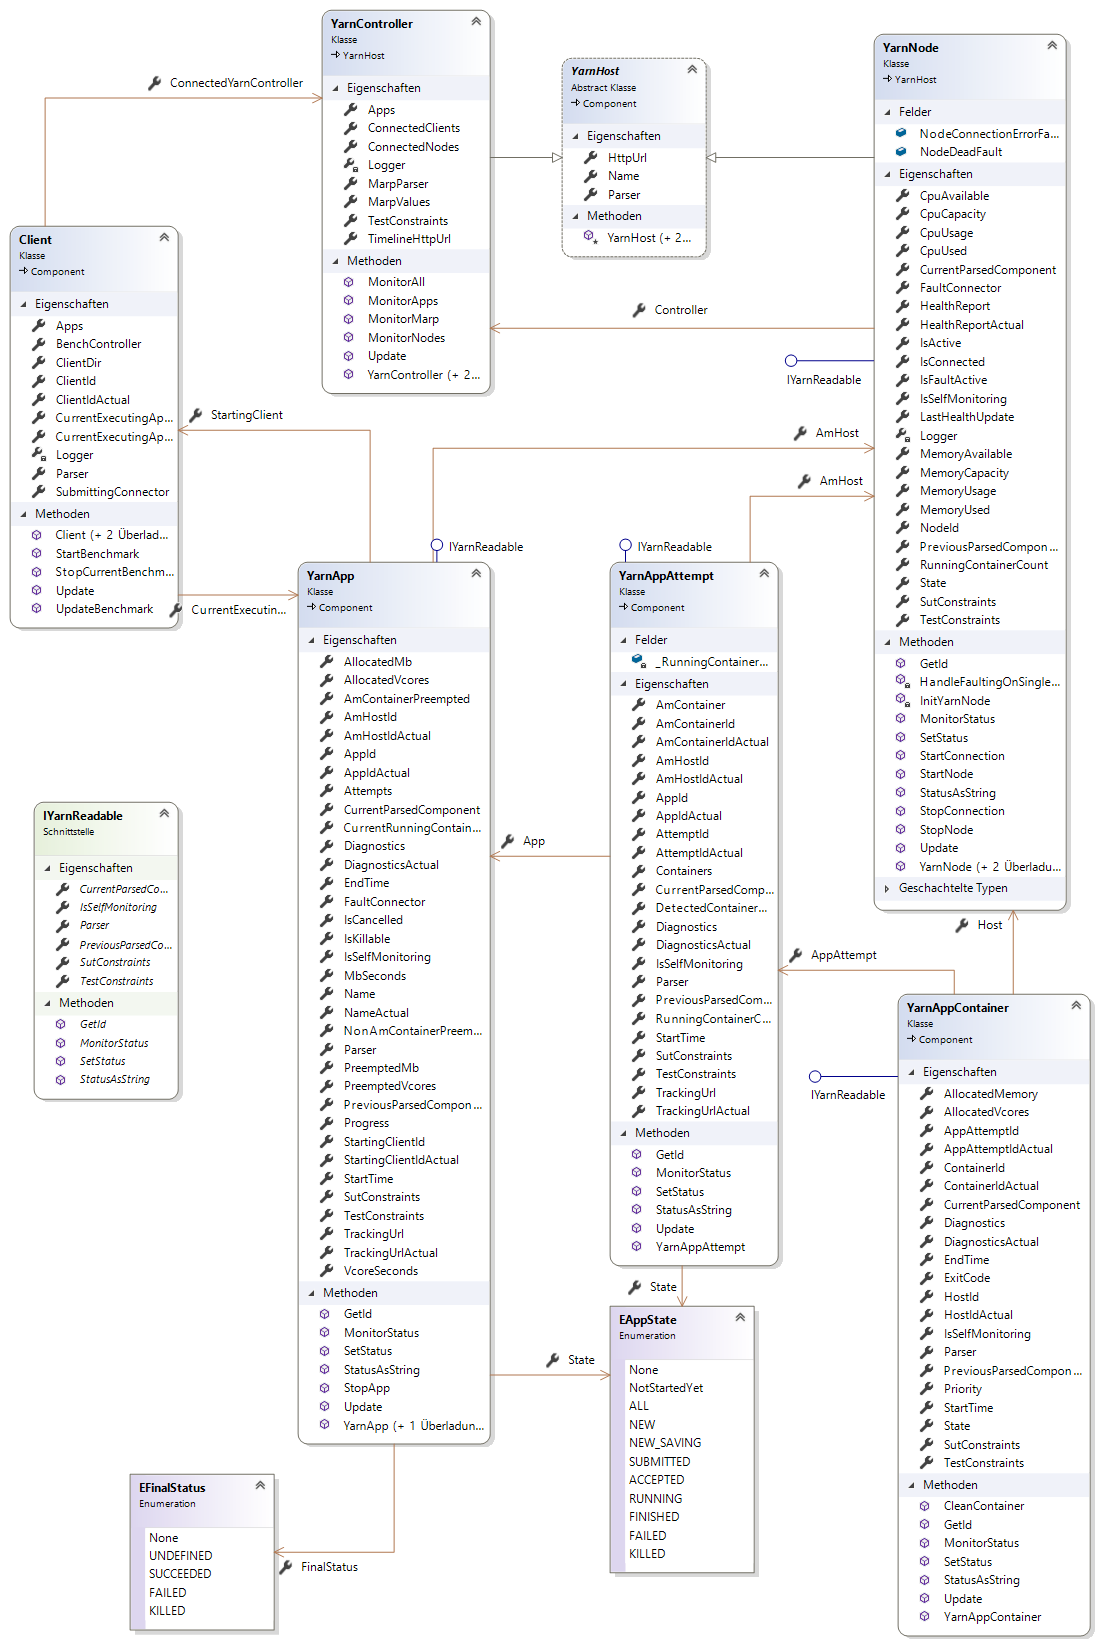
\includegraphics[width=\columnwidth]{./images/yarnModel.png}
	\caption[Aufbau des YARN-Modells]{Aufbau des YARN-Modells. Das Modell wurde mithilfe des Klassendiagramm-Designers in Visual Studio erstellt. Daher werden die aus Listen bestehenden Gegenverweise zu den Eigenschaften \texttt{YarnAppAttempt.App} und \texttt{YarnAppContainer.AppAttempt} nicht im Diagramm angezeigt.}
	\label{fig:yarnModel}
\end{figure}